\documentclass[12pt,a4paper]{scrbook}
\usepackage[utf8]{inputenc}
\usepackage[ngerman]{babel}
\usepackage{amsmath}
\usepackage{amsfonts}
\usepackage{amssymb}
\usepackage{graphicx}
\usepackage[bottom]{footmisc}
\usepackage[hidelinks]{hyperref}
\usepackage{color}
\author{\{Autoren hier vllt. einfügen\}}
\title{Mathematik 1. Kantonsschule}

\begin{document}
\shorthandoff{"}

\maketitle
\tableofcontents

\newpage

\chapter{Potenzgesetze}


\chapter{Strahlensätze und Ähnlichkeit}


\chapter{Funktionen}
\section{Definition einer Funktion}
Die Definition erfolgt durch eine Deklaration inklusive
der Zahlbereichen und des Zahlbereiches des "Rückgabewertes" der Funktion:

\[ f : \mathbb{R} \rightarrow \mathbb{R}\]
\[ f(x) = \frac{3}{7} + a^2 - \frac{b}{3x} + 2; \quad\quad x \in \mathbb{Z}\backslash\{0\}\]

\section{Lineare Funktion}
\subsection{Typische Definition}
\[f(x) = y = k \cdot x + d; \quad\quad k, d \in \mathbb{R}\]
\subsection{Lösungsformel}
\[x = \frac{-d}{k}\]

\subsection{Beispiel}
\[f(x) = -\frac{3}{2}x + 6\]

\subsection{Wertetabelle} der Funktion $f(x)$ wobei $x \in [-3; 7]$\\\\
\begin{tabular}{l||c|c|c|c|c|c|c|c|c|c|c}
$x$ & -3 & -2 & -1 & 0 & 1 & 2 & 3 & 4 & 5 & 6 & 7\\
\hline
$f(x)$ & 10.5 & 9 & 7.5 & 6 & 4.5 & 3 & 1.5 & 0 & -1.5 & -3 & -4.5\\
\end{tabular}\\\\\\
\textbf{Beachte:} $\Delta x$ ist konstant $-1.5$.\\

\subsection{Steigung}
\[f(x) = k\cdot x + d; \quad\quad k,d \in \mathbb{R}\]
$d$ ist der y-Achsenabschnitt. An diesem Ort wird die y-Achse\\
geschnitten. $k$ ist die Steigung von f.\\\\\\
\begin{tabular}{ll}
Wenn $k \geq 0$: & f ist wachsend\\
Wenn $k < 0$: & f ist fallend\\
\end{tabular}

\subsection{Stufenformel}
Herleitung der Stufenformel:
\[f(x+1) = f(x) + k\]
\[f(x+1) - f(x) = k\]
\[f(x+\Delta x) = f(x) + \Delta x \cdot k\]
\[f(x+\Delta x) - f(x) = \Delta x \cdot k\]
\[f(x+\Delta x) - f(x) = k\]

\begin{center}
\fbox{\parbox{4cm}{\[\frac{\Delta y}{\Delta x} = k\]}}
\end{center}


\subsubsection{Deutung der Steigung k}
Die Steigung einer linearen Funktion entspricht der Änderung\\
der Funktionswerte, bei Vermehrung des Arguments um 1.

\section{Quadratische Funktion}
\subsection{Typische Definition}
\[f(x) = y = ax^2 + bx + c; \quad\quad a \in \mathbb{R}\backslash\{0\}; \;\; b, c \in \mathbb{R}\]
\subsection{Lösungsformel}
\[x_1 / x_2 = \frac{-b \pm \sqrt{b^2-4ac}}{2a} \]
\subsection{Beispiel}
\[f(x) = \frac{1}{2}x^2 - \frac{3}{4}x - \frac{7}{2}\]

\subsection{Wertetabelle} der Funktion $f(x)$ wobei $x \in [-3; 7]$\\\\
\begin{tabular}{l||c|c|c|c|c|c|c|c|c|c|c}
$x$ & -3 & -2 & -1 & 0 & 1 & 2 & 3 & 4 & 5 & 6 & 7\\
\hline
$f(x)$ & 3.25 & 0 & -2.25 & -3.5 & -3.75 & -3 & -1.25 & 1.5 & 5.25 & 10 & 15.75\\
\end{tabular}\\\\\\
\textbf{Beachte:} $\Delta x$ ist nicht konstant!\\


\chapter{Quadratische Gleichungen}
\label{quadratische_gleichungen}


\chapter{Lineare Gleichungssysteme}


\chapter{Logik}
\section{Aussagen}
\section{Logikoperatoren}

\chapter{Mengen}
\section{Mengenoperationen}

\chapter{Beweise}
\section{Direkte Beweise}

\section{Indirekte Beweise}

\section{Induktive Beweise}

\chapter{Darstellende Geometrie}
\section{Einführung}
\textbf{Grundproblem:} räumliche Figur $\Leftrightarrow$ ebene Zeichnung \\\\
Die Darstellende Geometrie schafft Grundlagen für die zeichnerische, ebene Darstellung räumlicher Objekte
und die zeichnerische Lösung räumlicher Probleme. In der Mathematik sind die
folgenden Abbildungsverfahren gebräuchlich:

\begin{itemize}
  \item Schrägbild
  \item Darstellung mit einem oder mehreren Rissen
\end{itemize}

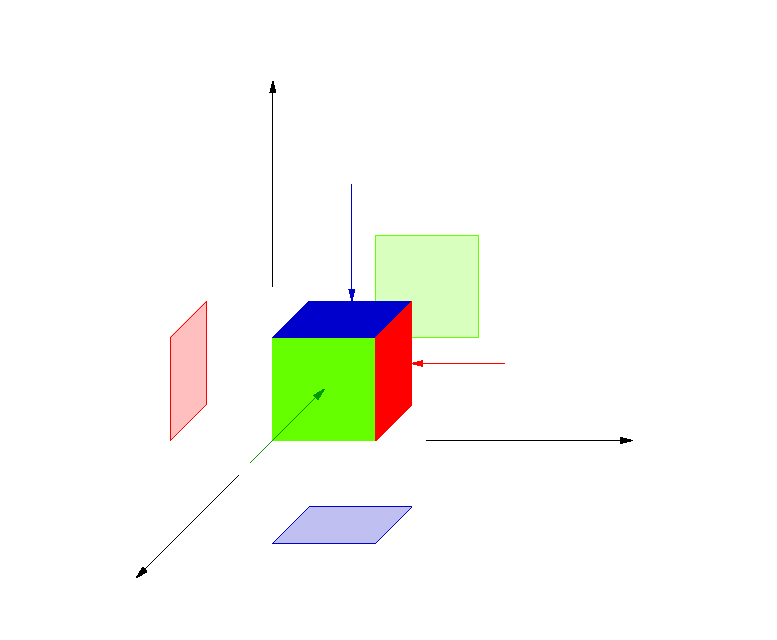
\includegraphics[scale=1]{img/einfuehrung.pdf}\\
\textcolor{blue}{Grundriss (Vogelperspektive)}\\
\textcolor{green}{Aufriss (Ansicht von vorne)}\\
\textcolor{red}{Seitenriss (Kreuzriss, Ansicht von der Seite)}

\section{Kavaliersprojektion}
\begin{figure}[h]
  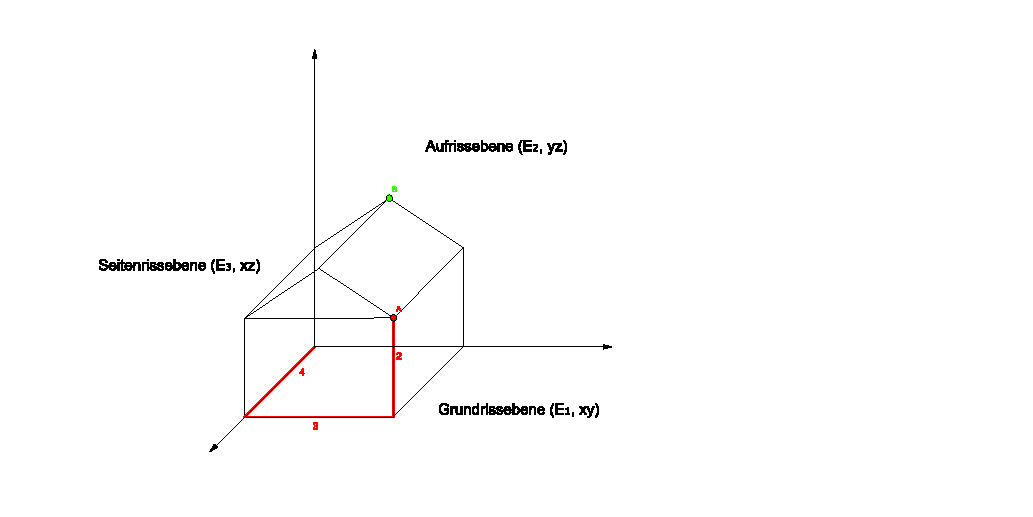
\includegraphics[scale=1.4]{img/einfuehrung_2.pdf}
  \caption{Beispiel: Haus in den vier üblichen Darstellungsarten}
\end{figure}

$a_{xy} = 135^{\circ}$

\section{Zweitafeldarstellung}
\section{Dreitafeldarstellung}

\chapter{Komplexe Zahlen}
\section{Grundlagen}
Während unserem ganzen Leben erweiteren wir unsere Zahlbereiche. Zuerst
reichten unsere natürlichen Zahlen von 0-10. Irgendwann kamen die Zahlen,
die grösser als 10 sind dazu ($\mathbb{N}$). Später entdeckten wir
negative Zahlen ($\mathbb{Z}^-$). Es kamen die rationalen Zahlen hinzu.
(z. Bsp. $\frac{1}{4} = 0.25 \in \mathbb{Q}$). Um alle möglichen Werte auf
der Zahlengerade bestimmen zu können (z. Bsp. $\sqrt{2} \in \mathbb{R}$)
beschrieb man die reellen Zahlen. Etwas später endeckte man, dass
gewisse Probleme nicht mehr in den reellen Zahlen lösbar sind.
Zum Beispiel einige quadratisch Gleichungen\footnote{Wie man quadratische Gleichungen lösen kann,
erfährt man auf Seite \pageref{quadratische_gleichungen}}
\begin{eqnarray*}
x^2+4 & = ~ 0\\
x^2+4x+13 & = ~ 0\\
x^2+1 & = ~ 0
\end{eqnarray*}
Deshalb wurden die komplexen Zahlen ($\mathbb{C}$) beschrieben. Die komplexen
Zahlen sind eine "Übermenge" der reellen Zahlen. Es gilt also:
\[\mathbb{N} ~ \subset ~ \mathbb{Z} ~ \subset ~ \mathbb{Q} ~ \subset ~ \mathbb{R} ~ \subset ~ \mathbb{C}\]

\section{Kartesische Darstellung}
Da wir auf unserem eindimensionalen Zahlenstrahl bereits alle Werte
beschreiben können, erweiteren wir den Strahl auf eine zweidimensionale
Ebene. Die x-Achse wird als die "reelle Achse" bezeichnet, wohingegen,
die neue hinzugekommene y-Achse "imaginäre Achse" genannt wird.\\
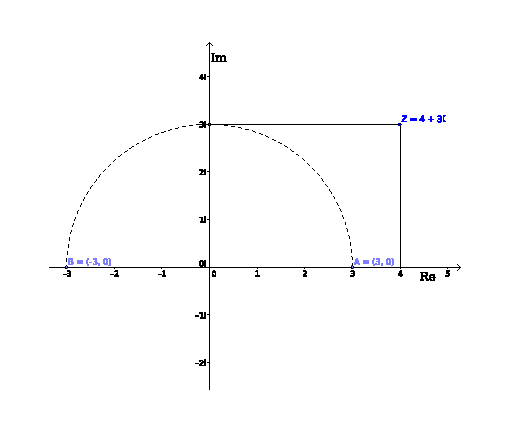
\includegraphics[scale=2]{img/komplexe_zahlen.pdf}\\
Das Problem der reellen Zahlen besteht darin, dass Wurzeln mit negativen
Radikanden unmöglich zu berechnen sind.

\section{Polardarstellung}


\section{Rechenoperationen}

\subsection{Addition}

\subsection{Subtraktion}

\subsection{Multiplikation}

\subsection{Division}

\subsection{Potenzen}

\section{Quadratische Gleichungen}

\section{Lineare Gleichungssysteme}


\end{document}
